% Class Notes Template
\documentclass[12pt]{article}
\usepackage[margin=1in]{geometry}
\usepackage[utf8]{inputenc}

% Packages
\usepackage{amsmath, amsthm, amssymb ,amsfonts, graphics, tikz, float, enumerate}
\usepackage{listings,verbatim, setspace}
\usepackage{booktabs}
\usepackage{siunitx}
\usepackage{color} %red, green, blue, yellow, cyan, magenta, black, white
\definecolor{mygreen}{RGB}{28,172,0} % color values Red, Green, Blue
\definecolor{mylilas}{RGB}{170,55,241}

\lstset{language=Matlab,%
	%basicstyle=\color{red},
	breaklines=true,%
	morekeywords={matlab2tikz},
	keywordstyle=\color{blue},%
	morekeywords=[2]{1}, keywordstyle=[2]{\color{black}},
	identifierstyle=\color{black},%
	stringstyle=\color{mylilas},
	commentstyle=\color{mygreen},%
	showstringspaces=false,%without this there will be a symbol in the places where there is a space
	numbers=left,%
	numberstyle={\tiny \color{black}},% size of the numbers
	numbersep=9pt, % this defines how far the numbers are from the text
	emph=[1]{for,end,break},emphstyle=[1]\color{blue}, %some words to emphasise
	%emph=[2]{word1,word2}, emphstyle=[2]{style},
}

\onehalfspacing

% Title
\title{ECON 7510 - Problem Set \#1}
\date{\today}
\author{Julien Manuel Neves}

% Use these for theorems, lemmas, proofs, etc.
\newtheorem{theorem}{Theorem}
\newtheorem{corollary}[theorem]{Corollary}
\newtheorem{lemma}[theorem]{Lemma}
\newtheorem{observation}[theorem]{Observation}
\newtheorem{proposition}[theorem]{Proposition}
\newtheorem{definition}[theorem]{Definition}
\newtheorem{claim}[theorem]{Claim}
\newtheorem{fact}[theorem]{Fact}
\newtheorem{assumption}[theorem]{Assumption}
\newtheorem{problem}[theorem]{Problem}
\newtheorem{set-up}[theorem]{Set-up}
\newtheorem{example}[theorem]{Example}
\newtheorem{remark}[theorem]{Remark}
\newtheorem{axiom}[theorem]{Axiom}

% Usefuls Macros
\newcommand{\field}[1]{\mathbb{#1}}
\newcommand{\N}{\field{N}} % natural numbers
\newcommand{\R}{\field{R}} % real numbers
\newcommand{\Z}{\field{Z}} % integers
\newcommand\F{\mathcal{F}}
\newcommand\B{\mathbb{B}}
\renewcommand{\Re}{\R} % reals
\newcommand{\Rn}[1]{\mathbb{R}^{#1}}
\newcommand{\1}{{\bf 1}} % vector of all 1's
\newcommand{\I}[1]{\mathbb{I}_{\left\{#1\right\}}} % indicator function
\newcommand{\La}{\mathscr{L}}
% \newcommand{\tends}{{\rightarrow}} % arrow for limits
% \newcommand{\ra}{{\rightarrow}} % abbreviation for right arrow
% \newcommand{\subjectto}{\mbox{\rm subject to}} % subject to

%% math operators
\DeclareMathOperator*{\argmin}{arg\,min}
\DeclareMathOperator*{\argmax}{arg\,max}
\DeclareMathOperator*{\maximize}{maximize}
\DeclareMathOperator*{\minimize}{minimize}
\DeclareMathOperator{\E}{\mathbb{E}} % expectation
\newcommand{\Ex}[1]{\E\left\{#1\right\}} % expectation with brackets
\DeclareMathOperator{\pr}{\mathsf{P}} % probability
\newcommand{\prob}[1]{\pr\left\{#1\right\}}
\DeclareMathOperator{\subjectto}{{s.t.\ }} % subject to
\newcommand{\norm}[1]{\left\|#1\right\|}
\newcommand{\card}[1]{\left|#1\right|}

% Extra stuff
\newcommand\seq[1]{\{ #1 \}}
\newcommand{\inp}[2]{\langle #1, #2 \rangle}

\newcommand{\inv}{^{-1}}

\newcommand{\pa}[1]{\left(#1\right)}
\newcommand{\bra}[1]{\left[#1\right]}
\newcommand{\cbra}[1]{\left\{ #1 \right\}}

\newcommand{\pfrac}[2]{\pa{\frac{#1}{#2}}}
\newcommand{\bfrac}[2]{\bra{\frac{#1}{#2}}}

\newcommand{\mat}[1]{\begin{matrix}#1\end{matrix}}
\newcommand{\pmat}[1]{\pa{\mat{#1}}}
\newcommand{\bmat}[1]{\bra{\mat{#1}}}

\begin{document}

\maketitle

\section*{Part 1}

From the problem set description, we start by assuming that each consumer $i$
has utility for product $j$ as a function of price and product quality, $\delta_j$ of the following form
\[
u_{ij} =\delta_j -\alpha_i p_j
\]
where the distribution of consumer price sensitivity, $\alpha_i$, is exponential with parameter $\lambda = 4\cdot 10^{-6}$. We further assume that $\delta_j = x_j\beta +\xi_j$ and that $x_j$ is uncorrelated with $\xi_j$.

In this model, $i$ choose the $j$ that provides the highest utility. This implies that if $p_j>p_k$, we need $\delta_j>\delta_k$ otherwise no one would ever pick $j$. In the same vein, it is straightforward to see that the share of good $j$ will depend only on its close neighbors in the price dimension. Hence, before deriving the result, we sort the data from lowest to highest price.

As mentionned above, to determine $j$ share we only need to compare its $u_{ij}$ to $j-1$ and $j+1$. In fact, $i$ will choose $j$ if and only if
\[
u_{i,j}>u_{i,j-1} \text{ and } u_{i,j}>u_{i,j+1}
\]

This boils down to the following condition for $\alpha_i$
\[
\frac{\delta_{j+1}-\delta_{j}}{p_{j+1}-p_{j}}<\alpha_i<\frac{\delta_j-\delta_{j-1}}{p_j-p_{j-1}}
\]
and therefore the share of good $j$ is given by
\begin{align*}
	s_j&=\int_{\frac{\delta_{j+1}-\delta_{j}}{p_{j+1}-p_{j}}}^{\frac{\delta_j-\delta_{j-1}}{p_j-p_{j-1}}}f(x)dx\\
	& = F\left({\frac{\delta_j-\delta_{j-1}}{p_j-p_{j-1}}}\right) - F\left( {\frac{\delta_{j+1}-\delta_{j}}{p_{j+1}-p_{j}}}\right)
\end{align*}
where $F(x)= 1-e^{-\lambda x}$.

Since we know $s_j$ and $p_j$, we can recursively solve for $\delta_j$, by noting that the following relationship holds
\[
\ln\left(\sum_{k=0}^j s_k\right) = -\lambda \left({\frac{\delta_{j+1}-\delta_{j}}{p_{j+1}-p_{j}}}\right)
\]

Using our $\delta_j$, we can compute our estimate for $\beta$ with simple OLS since the problem assumes that $\Ex{x_j\xi_j}=0$. The results are stated in Table \ref{tab:vertical}.

\begin{table}[H]\centering
\caption{Vertical model - Demand side only}
\begin{tabular}{c c }
\toprule
 & \textbf{Demand side} \\
\midrule
(Intercept)         &     \num{1.4370 e+8} \\
    &      [\num{1.0166 e+8}  \num{1.8575 e+8}]      \\
Horsepower / Weight         &     \num{1.6125 e+9} \\
  &      [\num{7.9606 e+8}  \num{2.4291 e+9}]      \\
AC         &     \num{5.7044 e+7} \\
	     &      [\num{4.3411 e+7}  \num{7.0676 e+7}]      \\
Firms FE       &      Yes \\
            &     \\
\midrule
 N           &     131     \\
R$^{2}$           &       0.7195   \\
\bottomrule
\addlinespace[1ex]
$[\quad] $ 95\% confidence interval
\end{tabular}
 \label{tab:vertical}
\end{table}

Note that while the regression in Table \ref{tab:vertical} includes fixed effects for the firm, I simply don't report their values for the sake of conciseness. Moreover, it is clear from our estimate that the coefficients values are immense which makes them difficult to interpret.


\section*{Part 2}

For the model, if two goods, for example $j$ and $k$, have the same price and strictly positive shares then $\delta_k=\delta_j$. As such, we have $u_{ik}=u_{ij}$ for all consumer for good $j$ and $k$. If it were not the case, one good would have zero market share. This is a fairly extreme assumption.

Looking at Table \ref{tab:vertical_elasticities}, we can see that the model insinuates rather odd own and cross price elasticities.
\begin{table}[H]
	\centering
	\caption{Vertical model - Price elasticities}
	\resizebox{\columnwidth}{!}{%
\begin{tabular}{lllllllllll}
	\toprule
Car$\backslash$Car & 15      & 16      & 17                                & 18      & 19      &
20      & 21      & 22      & 23      & 24      \\
\midrule
15                     & -0.0948 & 0.0003  & 0                                 & 0       & 0       & 0       & 0       & 0       & 0       & 0       \\
16                     & 0.0003  & -0.0003 & 0.0000 & 0       & 0       & 0       & 0       & 0       & 0       & 0       \\
17                     & 0       & 0.0001  & -0.0671                           & 0.0673  & 0       & 0       & 0       & 0       & 0       & 0       \\
18                     & 0       & 0       & 0.0050                            & -0.0154 & 0.0104  & 0       & 0       & 0       & 0       & 0       \\
19                     & 0       & 0       & 0                                 & 0.0711  & -0.5703 & 0.4997  & 0       & 0       & 0       & 0       \\
20                     & 0       & 0       & 0                                 & 0       & 0.1349  & -0.1477 & 0.0126  & 0       & 0       & 0       \\
21                     & 0       & 0       & 0                                 & 0       & 0       & 0.0235  & -0.0438 & 0.0202  & 0       & 0       \\
22                     & 0       & 0       & 0                                 & 0       & 0       & 0       & 1.2703  & -1.8608 & 0.5881  & 0       \\
23                     & 0       & 0       & 0                                 & 0       & 0       & 0       & 0       & 0.0175  & -0.0180 & 0.0004  \\
24                     & 0       & 0       & 0                                 & 0       & 0       & 0       & 0       & 0       & 0.0001  & -0.0390\\
\bottomrule
\end{tabular}%
}
 \label{tab:vertical_elasticities}
\end{table}

This weird substitution pattern stems from the fact that cross price elasticities for any given good is going to be equal to zero apart from its direct price neighbors. It is straightforward to show this fact by noting that $s_j= F\left({\frac{\delta_j-\delta_{j-1}}{p_j-p_{j-1}}}\right) - F\left( {\frac{\delta_{j+1}-\delta_{j}}{p_{j+1}-p_{j}}}\right)$ is not a function of any price apart from $p_j$, $p_{j-1}$, and $p_{j+1}$.

Moreover, the own-price elasticities are pretty close to each other accross the price spectrum. This is not what we would expect in reality (people buying high-end cars should be less price sensitive than people buying low-end cars).

\section*{Part 3}

We know turn our attention to the supply side of our model. We are given the following equation for marginal cost $mc_j = x_j\gamma +\eta q_j +\omega_j$. Sadly, we don't have the actual value for the marginal cost. We can circumvent this issue by relating marginal cost to price by assuming some pricing strategy for the firms. As a matter of fact, these pricing strategy will result in a markup over marginal cost given by the following formulas:
\begin{itemize}
	\item Marginal cost pricing:
	\[
p_j = mc_j
	\]
	\item Single product firms:
	\[
p_j = mc_j +\Delta\inv s
	\]
	where $\Delta_{jk} = \left\{\mat{\frac{\partial s_j}{\partial p_k} & \text{if }j=k\\ 0 & \text{otherwise}}\right.$ and $s$ is the vector of shares.

	\item Multiproduct firms:
	\[
p_j = mc_j +\Delta\inv s
	\]
	where $\Delta_{jk} = \left\{\mat{\frac{\partial s_j}{\partial p_k} & \text{if }k\in \text{firm}(j)\\ 0 & \text{otherwise}}\right.$ and $s$ is the vector of shares.

	\item Perfect collusion:
	\[
p_j = mc_j +\Delta\inv s
	\]
	where $\Delta_{jk} = \frac{\partial s_j}{\partial p_k} $ and $s$ is the vector of shares.
\end{itemize}

From the previous question, it is easy to to compute $\Delta$ and therefore $mc_j$.

With this in mind, we can revert back to $mc_j = x_j\gamma +\eta q_j +\omega_j$ and estimate it like we would for $\delta_j = x_j\beta +\xi_j$. The only issue we are facing now is	the potential endogeneity of $q_j$.

To remedy the situation, we need to find an instrument for $q_j$. There is plenty potential instruments, but after playing around for a while, I decide to follow BLP and use $\sum_{k\in \text{firm}(j)}  (x_k-x_j)$ and $\sum_{k\not\in \text{firm}(j)} x_k$. To avoid any problem with collinearity and matrix inversion, I use the function \verb!licols()! to reduce our set of instruments $Z = [x_j,\sum_{k\in \text{firm}(j)}  (x_k-x_j), \sum_{k\not\in \text{firm}(j)} x_k]$ to a full column rank matrix. Note that the function \verb!create_iv()! includes the method from Gandhi and Houde (2018).

We can now define our moments equations:
\begin{align*}
	\Ex{\mat{Z \bmat{\xi_j \\ \omega_j}}} = 0
\end{align*}

Using these moments conditions, we can run a GMM estimation using the different pricing strategy by stacking $\xi_j$ and $\omega_j$. Results are given in Table \ref{tab:vertical_supply}.


\begin{table}[H]\centering
\caption{Vertical model - supply side}
\resizebox{\columnwidth}{!}{%
\begin{tabular}{c c c c c}
\toprule
 & \textbf{Marginal cost} & \textbf{Single product firms} & \textbf{Multiproduct firms} & \textbf{Collusion} \\
\midrule
Demand \\
(Intercept)         &     \num{1.4370 e+8} &     \num{1.4370 e+8}&     \num{1.4370 e+8}&     \num{1.4370 e+8} \\
    &      [\num{1.0166 e+8}  \num{1.8575 e+8}]   &      [\num{1.0166 e+8}  \num{1.8575 e+8}]   &      [\num{1.0166 e+8}  \num{1.8575 e+8}]   &      [\num{1.0166 e+8}  \num{1.8575 e+8}]      \\
Horsepower / Weight         &     \num{1.6125 e+9}         &     \num{1.6125 e+9}         &     \num{1.6125 e+9}         &     \num{1.6125 e+9} \\
  &      [\num{7.9606 e+8}  \num{2.4291 e+9}]    &      [\num{7.9606 e+8}  \num{2.4291 e+9}]    &      [\num{7.9606 e+8}  \num{2.4291 e+9}]    &      [\num{7.9606 e+8}  \num{2.4291 e+9}]      \\
AC         &     \num{5.7044 e+7}   &     \num{5.7044 e+7}  &     \num{5.7044 e+7}  &     \num{5.7044 e+7} \\
	     &      [\num{4.3411 e+7}  \num{7.0676 e+7}]   &      [\num{4.3411 e+7}  \num{7.0676 e+7}]   &      [\num{4.3411 e+7}  \num{7.0676 e+7}]   &      [\num{4.3411 e+7}  \num{7.0676 e+7}]      \\
Firms FE       &      Yes &      Yes&      Yes&      Yes\\
            &     \\
\midrule
 N           &     131 &     131 &     131 &     131     \\
R$^{2}$           &       0.7195  &       0.7195 &       0.7195 &       0.7195  \\
	\midrule\\
	Supply
	(Intercept)         &     \num{-1.4439 e+4}  &     \num{2.1439 e+8} &     \num{2.4358 e+8} &     \num{3.3766 e+11} \\
 &      [\num{-4.1412 e+7}  \num{1.2534 e+4}]       &      [\num{-3.2494 e+8}  \num{7.5373 e+8}]     &      [\num{-4.4677 e+8}  \num{9.3394 e+8}]     &      [\num{2.8871 e+11}  \num{3.8660 e+11}]    \\
Horsepower/Weight         &     \num{4.9504 e+5}    &     \num{6.9673 e+8}    &     \num{1.0852 e+9}    &     \num{2.3462 e+12} \\
 &      [\num{2.2007 e+5}  \num{7.7001 e+5}] &      [\num{-4.8014 e+9}  \num{6.1948 e+9}]  &      [\num{-5.9525 e+9}  \num{8.1229 e+9}]  &      [\num{1.8472 e+12}  \num{2.8451 e+12}]       \\
	AC         &     \num{1.0480 e+4}    &     \num{-1.0186 e+8}   &     \num{-1.2394 e+8}   &     \num{6.2855 e+10}\\
		     &      [\num{4.1786 e+3}  \num{1.6781 e+4}]   &      [\num{-2.2786 e+8}  \num{2.4142 e+7}]  &      [\num{-2.8523 e+8}  \num{3.7338 e+7}]  &      [\num{5.1420 e+10}  \num{7.4290 e+10}]     \\
Quantity         &     \num{0.0301}  &     \num{-2070.9} &     \num{-2516.3} &     \num{1.0040 e+6} \\
 &      [\num{-0.1135}  \num{0.1736}]       &      [\num{-4.9414 e+3}  \num{799.5432}]     &      [\num{-6190.5}  \num{1158.0}]     &      [\num{7.4347 e+5}  \num{1.2645 e+6}]    \\

Firm	FE       &      Yes & Yes & Yes & Yes \\
						            &     \\
\midrule
 N           &     131 &     131 &     131 &     131     \\
R$^{2}$           &   0.8032 & 0.3507 &0.3821 &  0.8279   \\
\bottomrule
\addlinespace[1ex]
$[\quad] $ 95\% confidence interval
\end{tabular}%
}
 \label{tab:vertical_supply}
\end{table}

Note that the coefficients are all over the place, and it is not worth it to interpret them. Seems like our data set does not contain enough information to identify most of the parameters.


\section*{Part 4}

Potentially what we would want to identify the different pricing strategy would be some sort of shock on the supply side. For example, the exogeneous entry or exit of some product. Then, we could test which pricing equation fares better.

Short of this, we could simply run some goodness of fit test to help us select the best approximation. For example, we could start with the null hypothesis that firm use marginal cost pricing and compute the likelihood ratio statistic of the other pricing decision. Rejection of the null would imply that the firms have potentially some market power that can be explained by some Nash-Bertrand equilibrium.


\section*{Part 5}

We now assume that each consumer $i$ has utility for product $j$ as a function of price and product quality, $\delta_j$ of:
\[
u_{ij} =\delta_j +\epsilon_{ij}
\]
where $\delta_j = x_j\beta -\alpha p_j+\xi_j$, $\xi_j$ is the unosbervable characteristics of good $j$ and $\epsilon_{ij}$ follows a type I extreme value distribution.

As shown in class, we have that the share of good $j$ is given by
\[
s_j = \frac{e^{\delta_j }}{1+\sum_k e^{\delta_k}}
\]
or, equivalently,
\[
\ln(s_j)-\ln(s_0) = x_j\beta -\alpha p_j+\xi_j
\]

Armed with this regression, we can now estimate $[\beta, \alpha]$. Like with the supply side, we now have some endogeneity problem. To solve this, we use the same set of instruments, $Z = [x_j,\sum_k |x_j - x_k|, \sum_k (x_j - x_k)^2]$, and run an IV regression to get back both $[\beta, \alpha]$ and $\xi$. The result from our IV regression are reported in Table \ref{tab:logit}.

Moreover, Table  \ref{tab:logit} includes the estimation of demand and supply parameters assuming Nash-Bertrand equilibrium with multiproduct firms. Recall that with multiproduct firms, Nash-Bertrand equilibrium yields
\[
p = mc + \Delta\inv s  = \Delta\inv s + x\gamma +\eta q +\omega
\]
where $\Delta_{jk} = \left\{\mat{\frac{\partial s_j}{\partial p_k} & \text{if }k\in \text{firm}(j)\\ 0 & \text{otherwise}}\right.$ and $s$ is the vector of shares. We can solve explicitly for $\Delta$ by noting that $\frac{\partial s_j}{\partial p_k}= \left\{\mat{ -\alpha s_j(1-s_j) & \text{if } j= k\\ \alpha s_js_k & \text{otherwise}}\right.$. Let $\Delta\inv s = b(\alpha)$ since, unlike the vertical model, it depends on $\alpha$ in a non-linear fashion.

We can now define our moments equations:
\begin{align*}
	\Ex{\mat{Z\xi_j \\ Z\omega_j}} = 0
\end{align*}
or, equivalently
\begin{align*}
	\Ex{\mat{Z(\delta_j - x_j\beta +\alpha p_j) \\ Z(p_j-b_j(\alpha)-x_j\gamma -\eta q_j)}} = 0
\end{align*}
where $Z$ is the set of instruments. Using these statcked moments conditions, we can use our usual GMM technique to estimate $\theta = [\alpha, \beta, \gamma, \eta]$. Since $\alpha$ enters non-linearly, to solve for it I use \verb!fmincon()! to minize the objective function with respect to $\alpha$ and then solve for the rest of parameters using least squares techniques.

The only issue that I'm facing now is how to compute the standard errors of our estimate. Since, $\alpha$ enters non-linearly, I need to find the gradient of $s_j$ with $\theta$ to be able to compute the GMM covariance matrix. Estimation results are reported in Table \ref{tab:logit}.

\begin{table}[H]\centering
\caption{Vertical model - supply side}
\resizebox{\columnwidth}{!}{%
\begin{tabular}{c c c}
\toprule
 & \textbf{Demand only} & \textbf{Multiple product firms} \\
\midrule
(Intercept)         &     \num{-6.6124}  &     \num{-6.7250}  \\
  	   &       [\num{-8.0979}  \num{-5.1270}] &      [\num{-8.0552}  \num{-5.3949}]                  \\
Horesepower/Weight         &     \num{-8.5267}    &     \num{-2.9597}     \\
	   &       [\num{-43.7682}  \num{26.7149}] &      [\num{-28.7903}  \num{22.8710}]                  \\
AC         &     \num{-0.3297}    &     \num{-0.2147}  \\
	  	   &       [\num{-0.9764}  \num{0.3169}] &      [\num{-0.6459}  \num{0.2166}]                  \\
Price ($\alpha$)         &     \num{2.7842 e-5}    &     \num{4.0202 e-5}  \\
			 		   &       [\num{-2.1040 e-5}  \num{7.6723 e-5}] &      [\num{3.8732 e-5}  \num{4.1672 e-5}]                  \\
FE       &      Yes & Yes \\
            &     \\
\midrule
 N           &     131 &     131      \\
R$^{2}$          & 0.5696 &       0.5134   \\
	\midrule

	(Intercept)         &     &     \num{1.0631 e+4}  \\
	   &       &      [\num{-1.6342 e+4}  \num{3.7604 e+4}]                  \\
	Horesepower/Weight       &  &     \num{4.9504 e+5}     \\
	 	   &       &      [\num{2.2007 e+5}  \num{7.7001 e+5}]                  \\
	AC         &         &     \num{1.0480 e+4}  \\
		 	   &       &      [\num{4.1786 e+3}  \num{1.6781 e+4}]                  \\
	Quantity         &       &     \num{0.0301}  \\
			   &    &      [\num{-0.1135}  \num{0.1736}]                  \\
	FE       &   & Yes  \\
						            &     \\
\midrule
 N           &     131 &     131      \\
R$^{2}$           &&       0.8017   \\
\bottomrule
\addlinespace[1ex]
$[\quad] $ 95\% confidence interval
\end{tabular}%
}
 \label{tab:logit}
\end{table}

Again, we report the elasticities for a subset of the product in Table \ref{tab:logit_elasticities}.

\begin{table}[H]
	\centering
	\caption{Logit model - Price elasticities}
	\resizebox{\columnwidth}{!}{%
\begin{tabular}{lllllllllll}
	\toprule
Car$\backslash$Car & 15      & 16      & 17                                & 18      & 19      &
20      & 21      & 22      & 23      & 24      \\
\midrule
15                   & \num{-0.2057}  &  \num{6.2258e-04}  &  \num{4.1449e-5} &  \num{5.5583e-05} &  \num{8.1653e-05 }&  \num{3.0235e-4 }&  \num{1.6152e-04} &  \num{2.5681e-06} &  \num{8.6135e-05} &  \num{3.2681 e-4} \\
16                   &  \num{5.9558e-04} &  \num{-0.2103}   &  \num{4.1449e-5} &  \num{5.5583e-05} &  \num{8.1653e-05 }&  \num{3.0235e-4 }&  \num{1.6152e-04} &  \num{2.5681e-06} &  \num{8.6135e-05} &  \num{3.2681 e-4} \\
17                   &  \num{5.9558e-04} &  \num{6.2258e-04}  &  \num{-0.2420}  &  \num{5.5583e-05} &  \num{8.1653e-05}&  \num{3.0235e-4 }&  \num{1.6152e-04} &  \num{2.5681e-06} &  \num{8.6135e-05} &  \num{3.2681 e-4} \\
18                   &  \num{5.9558e-04} &  \num{6.2258e-04}  &  \num{4.1449e-5} &  \num{-0.2430  }&  \num{8.1653e-05 }&  \num{3.0235e-4 }&  \num{1.6152e-04 }&     \num{ 2.5681e-06} &  \num{8.6135e-05} &  \num{3.2681 e-4} \\
19                   &  \num{5.9558e-04} &  \num{6.2258e-04}  &  \num{4.1449e-5} &  \num{5.5583e-05}&  \num{-0.2445  }&   \num{3.0235e-4 }&  \num{1.6152e-04}&  \num{2.5681e-06} &  \num{8.6135e-05} &  \num{3.2681 e-4} \\
20                   &  \num{5.9558e-04} &  \num{6.2258e-04}  &  \num{4.1449e-5} &  \num{5.5583e-05 }&  \num{8.1653e-05}&  \num{-0.2447  }&  \num{1.6152e-04} &  \num{2.5681e-06} &  \num{8.6135e-05} &  \num{3.2681 e-4} \\
21                   &  \num{5.9558e-04} &  \num{6.2258e-04}  &  \num{4.1449e-5} &  \num{5.5583e-05 }&  \num{8.1653e-05}&  \num{3.0235e-4 }&  \num{-0.2461  }&  \num{2.5681e-06} &  \num{8.6135e-05} &  \num{3.2681 e-4} \\
22                   &  \num{5.9558e-04} &  \num{6.2258e-04} &  \num{4.1449e-5} &  \num{5.5583e-05 }&  \num{8.1653e-05 }&  \num{3.0235e-4 }&  \num{1.6152e-04 }&  \num{-0.2476}  &  \num{8.6135e-05} &  \num{3.2681 e-4} \\
23                   &  \num{5.9558e-04} &  \num{6.2258e-04 } &  \num{4.1449e-5} &  \num{5.5583e-05} &  \num{8.1653e-05 }&  \num{3.0235e-4 }&  \num{1.6152e-04 }&  \num{2.5681e-06} &  \num{-0.2496}  &  \num{3.2681 e-4} \\
24                   &  \num{5.9558e-04} &  \num{6.2258e-04} &  \num{4.1449e-5} &  \num{5.5583e-05}&  \num{8.1653e-05 }&  \num{3.0235e-4 }&  \num{1.6152e-04}&  \num{2.5681e-06} &  \num{8.6135e-05} &  \num{-0.2629}  \\

 \hline
\bottomrule
\end{tabular}%
}
 \label{tab:logit_elasticities}
\end{table}

Looking at these elasticities, we have an improvment compared to the previous vertical model where most cross price elasticities where equal to 0. But now, we the drawbacks of logit model, i.e. IIA property. This implies that odds of choosing some good $j$ over $k$ does not depend on other alternatives which is at odd with what we expect.

Notice that the own price elasticity of good $j$ depends solely on the price and share of $j$, while the cross price elasticities of $j$ depends on the price and share of $k$. Therefore, two goods with the same shares will have the same cross price elasticities for any other good and the same markup. Moreover, it is clear to see that from the cross price elasticities in Table \ref{tab:logit_elasticities} that an increase in price for some good $k$ will push consumer towards the most bought good. This is fairly odd as we don't expect people buying expensive car to switch to cheap cars if the price of high end cars rise slightly.



\section*{Part 6}

All three proposed model could improve our substitution patterns. First, the Pure Characteristics model assume away the logit error term $\epsilon_{ij}$. Since this is the source of the IIA problem with the logit model, it is straightforward to see that the Pure Characteristics model would improve our elasticities.

Moreover, the Nested Logit can be use to break the IIA by allowing correlation between some choices. For example, we could put high-end cars in the same nest to better capture how consumer choose between alternatives. In the same fashion, the Multinomial probit can also break IIA by allowing correlation between the error terms. In both cases, we improve on the substitution pattern.


\section*{Part 7}


We now assume that each consumer $i$ has utility for product $j$ as a function of price and product quality, $\delta_j$ of:
\[
u_{ij} =\delta_j-\alpha_i p_j+\epsilon_{ij}
\]
where $\delta_j = x_j\beta +\xi_j $, $\epsilon_{ij}$ follows a type I extreme value distribution and $\alpha_i = \frac{1}{y_i}$ where $y_i$ is income and distributed as a lognormal.

As shown in class, we have that the share of probability that $i$ buys good $j$ is given by
\[
P_{ij} = \frac{e^{\delta_j -\alpha_i p_j }}{1+\sum_k e^{\delta_k-\alpha_i p_k}}
\]

To obtain the shares, we need to integrate over the consumers, i.e.
\[
g_j = \int \frac{e^{\delta_j -\alpha_i p_j }}{1+\sum_k e^{\delta_k -\alpha_i p_k}} d\Phi(\alpha_i)
\]
where $\Phi(\cdot)$ is the lognormal distribution of income. In our context, it might be easy to integrate out the probabilities since we only have one $\alpha_i$ and that the lognormal is fully characterize by its two unknown parameters $\mu$ and $\sigma$. Usually, it is easier to simulate the $\alpha_i$ and take average of the probabilities. This is what we do in this problem set, by simulating $ns$ $y_i$ from a lognormal with $\mu$ and $\sigma$ and solving for $g_j$ with the following formula:
\[
g_j= \frac{1}{ns}\sum_{i=1}^{ns}\frac{e^{\delta_j -\alpha_i p_j }}{1+\sum_k e^{\delta_k -\alpha_i p_k}}
\]

With the $s_j$ in hands, we need to find the parameters to match them to the data. To do this, we first pick some $\mu$ and $\sigma$. Next, we solve for $\delta_j$ with a fixed point iteration
\[
\delta^{l+1} = \delta^{l} + \ln(s)-\ln(g_j)
\]

Recalling that $\delta_j = x_j\beta +\xi_j $, it is easy to see that we can solve for our unknowns by using the following moment condition $\Ex{\xi_j\mid Z}=0$ or
\[
\Ex{Z\xi_j } =0
\]
where $Z$ is the set of instruments as defined previously. Note that $\xi_j$ depends on $\beta$ linearly since $\xi_j = \delta_j(\mu,\sigma)-x_j\beta$, but it depends on $\sigma$ and $\mu$ we depend on them to find $\delta_j$. Therefore, given $\mu$ and $\sigma$ we can solve for $\beta$ and $\xi_j$ using least squares, but we can't use the same technique to solve for the non-linear parameters.

Therefore, what we do to solve for $\mu$ and $\sigma$ is to minimize the following objective function
\[
(Z'\xi(\mu,\theta))'W(Z'\xi(\mu,\sigma))
\]
where $W$ is some weighting matrix. In this problem, we let $W=Z'Z$ which is optimal if the $\xi_j$ are homoskedastic.

To solve for this problem, we can simply use any optimization algorithm to minize the objective function.

Now, suppose that $\alpha_i = \alpha_1 + \frac{\alpha_2}{y_i}$. The first thing to note is that $\alpha_1$ will enter $\delta_j$ linearly, and we can brush it aside as it is easy to deal with this. As for $\alpha_2$, it simply an added non-linear parameter to deal with and we can take care of it like $\mu$ and $\sigma$.

The question that remains is, can we identify our parameters. Technically, if we have more instruments than parameters we should be in the clear. Past this requirement, we may face two problems. First, we might not have enough variation and power to identify both $[\beta, \alpha]$ and $[\alpha_2, \mu, \sigma]$. Second, since $Y_i=\frac{\alpha_i}{y_i}$ can be seen as a random variable, depending on the functional form of its distribution it might be simply impossible to seperatly identify all three parameters $[\alpha_2, \mu, \sigma]$.

\section*{Part 8}

The estimation results for the model described in part 7 are reported in Table \ref{tab:blp}.

\begin{table}[H]\centering
\caption{BLP model - supply side}
\begin{tabular}{c c c}
\toprule
(Intercept)         &     \num{-6.6124}  \\
  	   &       [\num{-8.0967}  \num{-5.1281}]                  \\
Horesepower/Weight         &     \num{-8.5261}      \\
	   &       [\num{-43.7403}  \num{26.6881}]                \\
AC         &     \num{-0.3297}      \\
	  	   &       [\num{-0.9758}  \num{0.3165}]               \\
Price ($\alpha_!$)         &     \num{2.7433 e-5}   \\
			 		   &       [\num{-2.1410 e-5}  \num{7.6276 e-5}]                 \\
Price ($\alpha_2$)         &     \num{0.0057}  \\
					 		   &       [\num{-0.8140}  \num{0.8255}] \\
FE       &      Yes  \\
            &     \\
\midrule
 N           &     131       \\
R$^{2}$           &   0.5687    \\
\bottomrule
\addlinespace[1ex]
$[\quad] $ 95\% confidence interval
\end{tabular}
 \label{tab:blp}
\end{table}

It is important to note that for different starting value for our minimization algorithm, we find different value for $\alpha_2$ and hence different $[\beta, \alpha_1]$. Figure \ref{fig:alpha2} shows an histogram of the different values of $\alpha_2$ obtained with a 100 starting point evenly spaced between 0 and 50.

\begin{figure}
	\centering
	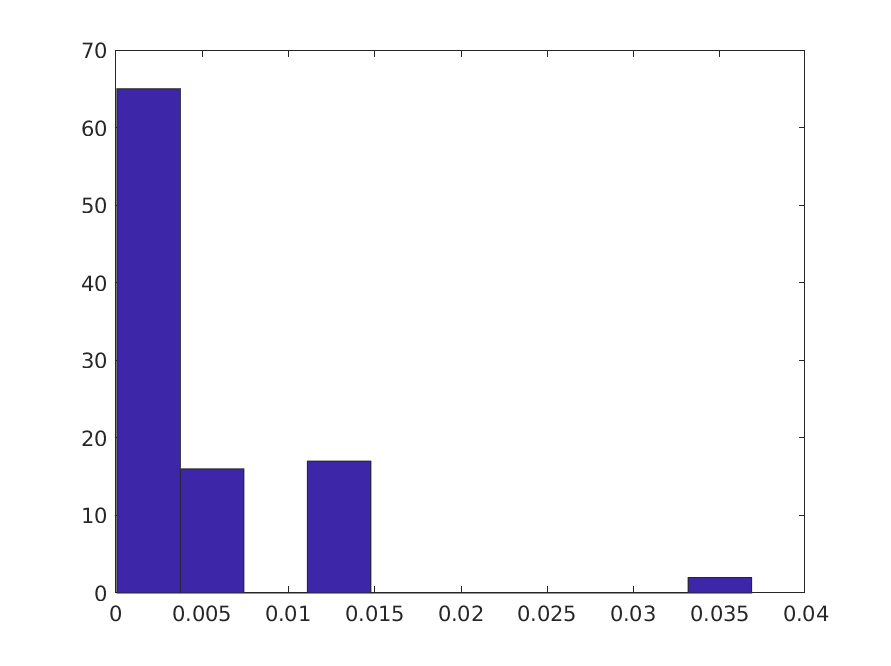
\includegraphics[width=0.7\linewidth]{../output/alpha2}
	\caption{histogram of $\alpha_2$ for different starting value}
	\label{fig:alpha2}
\end{figure}

Finally, we can look at the prices elasticities implied by the model as shown in Table \ref{tab:blp_elasticities}.
\begin{table}[H]
	\centering
	\caption{BLP model - Price elasticities}
	\resizebox{\columnwidth}{!}{%
\begin{tabular}{lllllllllll}
	\toprule
Car$\backslash$Price & 15      & 16      & 17                                & 18      & 19      &
20      & 21      & 22      & 23      & 24      \\
\midrule
15                   & \num{-0.2006}  &  \num{6.1943e-04}  &  \num{4.1220e-05} &  \num{5.5274e-05} &  \num{8.1199e-05 }&  \num{3.0067e-04 }&  \num{1.6062e-04} &  \num{2.5537e-06} &  \num{8.5649e-05} &  \num{3.2490e-04} \\
16  &  \num{5.9257 e-4} &  \num{-0.2098}   &  \num{4.1217 e-5} &  \num{5.5270e-4} &  \num{8.1193e-5}&  \num{3.0065e-4}&  \num{1.6061e-4} &  \num{2.5535 e-6} &  \num{8.5643 e-5} &  \num{3.2488e-4} \\
17  &  \num{5.9229 e-4} &  \num{6.1909 e-4}   &  \num{-0.2413} &  \num{5.5244e-4} &  \num{8.1155e-5}&  \num{3.0051e-4}&  \num{1.6053e-4} &  \num{2.5523 e-6} &  \num{8.5603 e-5} &  \num{3.2472e-4} \\
18  &  \num{5.9228 e-4} &  \num{6.1908 e-4}   &  \num{4.1197 e-5} &  \num{-0.2423} &  \num{8.1153e-5}&  \num{3.0050e-4}&  \num{1.6053e-4} &  \num{2.5523 e-6} &  \num{8.5601 e-5} &  \num{3.2472e-4} \\
19  &  \num{5.9227 e-4} &  \num{6.1907 e-4}   &  \num{4.1196 e-5} &  \num{5.5242e-4} &  \num{-0.2438}&  \num{3.0050e-4}&  \num{1.6052e-4} &  \num{2.5522 e-6} &  \num{8.5600 e-5} &  \num{3.2471e-4} \\
20  &  \num{5.9226 e-4} &  \num{6.1907 e-4}   &  \num{4.1196 e-5} &  \num{5.5242e-4} &  \num{8.1151e-5}&  \num{-0.2440}&  \num{1.6052e-4} &  \num{2.5522e-6} &  \num{8.5599 e-5} &  \num{3.2471e-4} \\
21  &  \num{5.9225 e-4} &  \num{6.1905 e-4}   &  \num{4.1195 e-5} &  \num{5.5241e-4} &  \num{8.1150e-5}&  \num{3.0049e-4}&  \num{-0.2454} &  \num{2.5522 e-6} &  \num{8.5597 e-5} &  \num{3.2470e-4} \\
22  &  \num{5.9224 e-4} &  \num{6.1904 e-4}   &  \num{4.1194 e-5} &  \num{5.5240e-4} &  \num{8.1148e-5}&  \num{3.0048e-4}&  \num{1.6052e-4} &  \num{-0.2469} &  \num{8.5596 e-5} &  \num{3.2470e-4} \\
23  &  \num{5.9222 e-4} &  \num{6.1902 e-4}   &  \num{4.1193 e-5} &  \num{5.5238e-4} &  \num{8.1145e-5}&  \num{3.0047e-4}&  \num{1.6051e-4} &  \num{2.5520 e-6} &  \num{-0.2489} &  \num{3.2469e-4} \\
24  &  \num{5.9210 e-4} &  \num{6.1889 e-4}   &  \num{4.1185 e-5} &  \num{5.5226e-4} &  \num{8.1129e-5}&  \num{3.0041e-4}&  \num{1.6048e-4} &  \num{2.5515 e-6} &  \num{8.5575 e-5} &  \num{-0.2621} \\
\bottomrule
\end{tabular}%
}
 \label{tab:blp_elasticities}
\end{table}

It is clear now that we have slightly improved the pattern of substitution between goods. In fact, unlike the simple logit model, our new elasticities do not satisfy the IIA property which is what we desired. On the otherhand, the few data points we have and the lack of micro-moments does not help us.


\section*{Part 9}

Recall that we assume that each consumer $i$ has utility for product $j$ as a function of price and product quality, $\delta_j$ of:
\[
u_{ij} = x_j\beta +\xi_j -\alpha p_j+\epsilon_{ij}
\]
where $\epsilon_{ij}$ follows a type I extreme value distribution and $\alpha = \alpha_1 + \frac{\alpha_2}{y_i}$ where $y_i$ is income and distributed as a lognormal.

The micro-moments presented in the problem set can supplement our model by observing that the taste preference for some characteristics (Horesepower to weight) a function of individual specific characteristics. In our context, we account for this by modifying our $\beta$ to include this possibility, i.e.
\[
\beta_{i,hp/w} = \beta_{hp/w} + y_{i}\beta_{hp/w}^0
\]
where $\beta_{hp/w}^0$ is the preference associated with observed consumer attributes.

Note that we could also include some unobservable idiosyncratic tastes in $\beta_{i,k}$.

Then, as previously described, our first moment is still the one that matches market shares. The new moment condition is given by
\[
G^2(\theta) = \sum_j \frac{n_j}{ns} x_{j,hp/w} \cbra{ \frac{1}{n_j}\sum_i y_i - \Ex{y \mid j , \theta} } - 0.7 \sigma_y \sigma_{x_{hp/w}} = 0
\]
where $n_j$ is the number of people that buy good $j$ and $\Ex{y \mid j , \theta}$ is the expected income of someone buying car $j$ given $\theta$ and $\sigma_y$ $\sigma_{x_{hp/w}}$ are variance of income and horesepower/weight. We can compute $\Ex{y \mid j , \theta}$ using Bayes' rule and the moment derive in the first part of the model.

While useful for the random coefficient model, micro-moments have no impact in the logit model since it ignore unobserved consumer preference. Hence, it would not be useful to estimate the parameters or change the substitution patterns in part 5.


\section*{Code}
\singlespace
\subsection*{Main file}
\lstinputlisting[language=Matlab]{run_me.m}
\subsection*{BLP\_model}
\lstinputlisting[language=Matlab]{blp_model.m}
\subsection*{create\_iv}
\lstinputlisting[language=Matlab]{create_iv.m}
\subsection*{get\_markup}
\lstinputlisting[language=Matlab]{get_markup.m}
\subsection*{get\_mean\_utility}
\lstinputlisting[language=Matlab]{get_mean_utility.m}
\subsection*{get\_shares}
\lstinputlisting[language=Matlab]{get_shares.m}
\subsection*{gmm\_fun}
\lstinputlisting[language=Matlab]{gmm_fun.m}
\subsection*{logit\_model}
\lstinputlisting[language=Matlab]{logit_model.m}
\subsection*{vertical\_model}
\lstinputlisting[language=Matlab]{vertical_model.m}
\subsection*{prepare\_data}
\lstinputlisting[language=Matlab]{prepare_data.m}


\end{document}
